Este capítulo está basado en los libros \textit{Monte -Carlo methods in financial engineering}, capítulo 1, P. Glasserman \cite{glass} y \textit{Processus de Markov et applications. Algorithmes, Réseaux, Génome et Finance}, capítulo 1, É. Pardoux\cite{pardoux}.
\subsubsection{Introducción}
Monte Carlo es un nombre común para varios métodos, cuyo elemento en común es el uso de la aleatoriedad, con la cual típicamente se usarán para  % simulaciones o algún cálculo numérico.
% La idea es:
\begin{itemize}
    \item calcular cantidades/integrales
    \item simular objetos matemáticos
\end{itemize}
Ambos deterministas, en base a números/objetos aleatorios.

\newp Los métodos de tipo Monte Carlo aparecen en variadas aplicaciones que incluyen: resolución de EDP, física, biología matemática, economía, ingeniería, finanzas, aprendizaje de máquinas, optimización, entre otras.
\newp Origen: 1940-1950 (Fermi, Ulam, Metropolis, Von Neumann) Relacionada a los avances en física nuclear: simulación computacional aleatoria de soluciones de la ecuación de fisión. 
\subsection{Descripción de M.C.}
\newp Consideremos la siguiente integral:
$$ I:=\displaystyle\int_\Omega f(x)m(dx) \, ,$$
con $\Omega\subset\Rd,m\in\mathcal{P}(\Omega)$ y $f\in L^1(m)$.

Estas integrales son \textbf{esperanzas}: $I=\E(f(X))$ si $X\sim m$.
En particular si $m$ tiene densidad $g$,
$$ \E(f(X)) = \displaystyle \int_\Omega f(x)g(x)dx \, .$$
Luego \textit{simulando} $\vas$ \textit{replicas} i.i.d $\sim m$ podemos aproximar $I$, por \textbf{ley de grandes números}
$$ \displaystyle\frac{1}{n}\sum^n_{k=1}f(X_k)\convcs I \, ,$$
y también en $L^p$ si $f(X_1)\in L^p, p\in[1,\infty)$.
\newp \textbf{¿Como se puede llevar a cabo esta simulación?}

Los computadores pueden producir secuencias pseudoaleatorias de números $U_1,U_2,\dots,U_n,\dots$ que ``parecen'' i.i.d. $\sim \mathbb{U}([0,1])$. En realidad , son secuencias deterministas a valores en una grilla discreta muy fina, generadas con un sistema dinámico discreto con un ciclo larguísimo a partir de una \textit{semilla} (seed) generada ``aleatoriamente''.

A partir de $U_1,U_2,\dots,U_n,\dots$ podemos generar (en teoría y en la práctica) v.a., $\vas$ i.i.d. en $R^d$ de ley $m$ cualquiera.

%\newp \textbf{¿Cómo generamos $\vas$ i.i.d. $\sim m$ más generales que la uniforme?}
%
%Veremos algunos métodos a continuación
%
\newp \textbf{¿Qué tan buena es la aproximación (aleatoria)} $\displaystyle\frac{1}{n}\sum^n_{k=1}f(X_k)\approx I=\E(Y_1)$?

Sabemos que si $Y_k:=f(X_k)\in L^2$, tenemos la siguiente \textbf{cota para el error cuadrático medio}:
$$ \E[|\displaystyle\frac{1}{n}\sum^n_{k=1}f(Y_k)-\E(Y_k)|^2]\leq\frac{\var(Y_1)}{n} \, .$$
En efecto,
\begin{alignat*}{2}
   \E(|\mean{(Y_k-I)}|^2) &  =  \displaystyle\frac{1}{n^2}\sum_{k=1}^n\E((Y_k-Y)^2)+\frac{1}{n^2}\sum_{j\neq k}\frac{\E((Y_k-I)(Y_j-I))}{\E(Y_k-I)\E(Y_j-I)} \\
     & = \displaystyle\frac{1}{n^2}\sum_{k=1}^n\E((Y_k-Y)^2)=\frac{\var(Y_n)}{n}
\end{alignat*}
% $$\E(|\mean{(Y_k-I)}|^2)=\displaystyle\frac{1}{n^2}\sum_{k=1}^n\E((Y_k-Y)^2)+\frac{1}{n^2}\sum_{j\neq k}\frac{\E((Y_k-I)(Y_j-I))}{\E(Y_k-I)\E(Y_j-I)}=\displaystyle\frac{1}{n^2}\sum_{k=1}^n\E((Y_k-Y)^2)=\frac{\var(Y_n)}{n}$$

Además por T.C.L. (\ref{tcl}), obtenemos \textbf{intervalos de confianza asintóticos}: Sean $Y_1,Y_2,\dots \iid\in L^2 $ e $I=\mu=\E(Y_1)$:
$$ \sqrt{n}(\bar{Y_n}-\mu)\convley\normal(0,\sigma^2) \, ,$$
con $\sigma^2=\var(Y_1)$. Y entonces para $n$ grande,
$$ \P(|\bar{Y}_n-\mu|\leq\displaystyle\frac{\sigma}{\sqrt{n}}Z_{\frac{\alpha}{2}})\approx 1-\alpha \, ,$$
con $\alpha\in(0,1)$ y $Z_{\frac{\alpha}{2}}$ tal que $\P(\normal(0,1)>Z_{\frac{\alpha}{2}})=\displaystyle\frac{\alpha}{2}$, donde hemos usado la caracterización \textit{(vi)} del Teorema de Portmanteau (\ref{portmanteau}).
\newp Entonces \textbf{para lograr una precisión $\epsilon$ con probabilidad $\geq1-\alpha$}, i.e., $$\P(|\hat{Y}_n-\mu|\leq \epsilon)\geq1-\alpha \, ,$$ \textbf{tenemos que tomar n tal que}:
$$ \displaystyle\frac{\sigma Z_{\frac{\alpha}{2}}}{\sqrt{n}}\leq\epsilon \espacio \ssi \espacio n \geq \frac{\sigma^2 Z^2_{\frac{\alpha}{2}}}{\epsilon^2} \, .$$
% \vspace{1cm}
\begin{remark}
\beforeitemize
\begin{itemize}
    \item El $n$ requerido para lograr una precisión $\epsilon$ dada no depende de la dimensión $d$, contrariamente a métodos deterministas, donde aproximar $\int_{[0,1}f(x)dx$ con precisión $\epsilon$ para $f$ Lipschitz requiere $\epsilon^{-d}$ evaluaciones, lo cual es impracticable para $d$ no pequeño ($>3$).
    \item El $n$ requerido para una precisión dada será mejor (más pequeño) si $\sigma^2$ es más pequeño. Esto es importante pues si disponemos de $Y_1,\dots,Y_n \mbox{ e } Y_1',\dots,Y_n' \iid \tq \E(Y_1)=\E(Y_1')=\mu$ y $\sigma^2=\var(Y_1)<\sigma^2'=\var(Y_1')$ entonces es preferible hacer M.C. con $Y_1,\dots,Y_n,\dots$ para aproximar $\mu$, siempre y cuando el costo de simular cada réplica de $Y_n$ y de $Y_n'$ sea similar.
    \item En general ¿cómo comparar entre dos M.M.C?\newline
    Consideremos:
    \begin{itemize}
        \item MC(1) v.a. $\iid Y_1,\dots,Y_n,\dots$ con costo $C$ por réplica
        \item MC(2) v.a. $\iid Y_1',\dots,Y_n',\dots$ con costo $C'$ por réplica
    \end{itemize}
    Para obtener una precisión $\epsilon>0$ con probabilidad $\geq 1-\alpha$ necesitamos alguno de los siguientes:
    $$ n\approx\nmc \mbox{ con MC(1) a costo total }Cn$$
    $$ n'\approx\displaystyle\frac{\sigma^2' Z^2_{\frac{\alpha}{2}}}{\epsilon^2}\mbox{ con MC(2) a costo total }C'n'$$
    Luego MC(1) es preferible a MC(2) ssi:
    $$ Cn<C'n'\ssi C\var(Y_1)<C'\var(Y'_1) \, .$$
    \item En general \textbf{no necesariamente conocemos} $\sigma^2=\var(Y_1)$, que es necesario para los análisis anteriores.
    \newline Sin embargo podemos estimarlo mediante una simulación \textit{piloto} (más pequeña y previa a calcular (I)) usando el estimador (insesgado):
    $$ \sigma^2\approx\displaystyle\frac{1}{q-1}\sum^q_{k=1}(\bar{Y}_q-Y_k)^2 \, ,$$
    con $q\approx10^2$ o $10^3$.
\end{itemize}
\end{remark}
\subsection{Simulación de variables aleatorias reales}  % clase 6 2 septiembre
Asumimos que podemos simular $(U_n)_{n\in\N} \iid \sim \unif$. Veremos como simular a partir de ellas realizaciones $(X_m)_{m\in \N}$ de v.a. de otras leyes. En teoría, basta una v.a. $\unif$ para simular variables aleatorias en cualquier espacio $(E,d)$ polaco. Más aún se tiene:
\begin{theorem}[de Representación de Skorokhod]
\label{sko}
Sean $X_n,n\in\N$, $X$ v.a. en $(E,d)$ polaco, tal que $X_n\convley X$. Entonces $\exists Y_n:[0,1]\to E,n\in\N$, $Y:[0,1]\to E$ medibles tal que si $U\sim\unif$,
$$ Y_n(U) \igualley X_n\mbox{,  } Y(U)\igualley X \mbox{ y }Y_n(U)\convcs Y(U) \, .$$
\end{theorem}
\begin{proof}
\gris En Billingsley \cite{billing} \negro
\end{proof}
\begin{remark}
Lamentablemente las funciones $Y_n,Y$ no son construibles.% (ver sección \ref{metgen}).
\\ En $E=\R$ si se pueden definir como $Y_n=F^{-}_{\mbox{ }X_n},Y=\Finvgen$, donde $F^-$ se será enunciado más adelante en definición \ref{def:invgen}.
\end{remark}
\vspace{2cm}\\
A continuación algunas \textbf{variables clásicas} que si se pueden simular con $\unif$.
\subsubsection{Bernoulli, Binomial y Geométrica}
\begin{definition}[Variable Bernoulli]
Sea $p\in(0,1)$ una v.a. Bernoulli $X$ puede realizarse como:
$$ X:=\mathbf{1}_{[0,p]}(U) \espacio \mbox{ con } \espacio U\sim\unif \, .$$
Esto se denota $ X\sim Ber(p)$.
\end{definition}
% Su \textbf{costo de simulación por réplica} está dado por:
% $$ C(Ber(p)) = C(U) + evaluación $$
\begin{definition}[Variable Binomial]
Sea $p\in(0,1),N\in\N$, una variable binomial $X$ está dada por:
$$ X:=\mathbf{1}_{[0,p]}(U_1)+\mathbf{1}_{[0,p]}(U_2)+\dots+\mathbf{1}_{[0,p]}(U_N)$$
Lo denotamos $X\sim Bin(p\,;N)$
\end{definition}
% Su \textbf{costo de simulación por réplica} está dado por:
% $$ C(Bin(p,N)) \approx N C(Ber(p)) \, .$$
\begin{definition}[Variable Geométrica]
Sea $p\in(0,1)$, decimos que $X$ es una variable geométrica si está dada por:
$$ X=\inf\{k\geq1:U_k\leq p\} \, .$$
Esto se denota $X\sim Geo(p)$
\end{definition}
% Su \textbf{costo de simulación por réplica} está dado por:
% $$ C(Geo(p)) \approx \displaystyle\frac{1}{p}C(Ber(p)) \, .$$
\begin{remark}[Costos de simulación por réplica]
Para las variables descritas anteriormente, los costos de simulación por réplica (denotado $C(\cdot)$) están dados por:
\begin{itemize}
    \item \textbf{Bernoulli}
    $$ C(Ber(p)) = C(U) + evaluación $$
    \item \textbf{Binomial}
    $$ C(Bin(p,N)) = N C(Ber(p))$$
    \item \textbf{Geométrica}
    % $$ C(Geo(p)) \approx \displaystyle\frac{1}{p}C(Ber(p)) $$
    $$ C(Geo(p)) = Geo(p)\cdot C(Ber(p))$$
\end{itemize}
El costo $C(Geo(p))$ es aleatorio, y lo aproximamos usando la esperanza:
% Agregar cosas % 43min clase 6
$$ Geo(p)\cdot C(Ber(p))\approx \E(Geo(p))C(Ber(p))=\displaystyle\frac{1}{p}C(Ber(p)) \, .$$
% \\ \textbf{¿Cómo estimar los costos de simulación por réplica?}
\\ \textbf{Además, para estimar el costo de simulación por réplica se puede proceder como sigue:}
\begin{enumerate}
    \item Simular $N(\approx100,1000)$ réplicas.
    \item Contar tiempo $T_N$ requerido.
    \item Costo/réplica $\approx \displaystyle\frac{T_N}{N}$.
\end{enumerate}
\end{remark}

\subsubsection{Variables reales generales}
Utilizaremos el \textbf{método de la inversa generalizada}.
\begin{definition}[Inversa generalizada]
\label{def:invgen}
Sea $X$ v.a. real, $F_X$ su función distribución. Definimos la inversa generalizada de $F_X:[0,1]\mapsto\R$,
$$ \Finvgen(t):=\inf\{x\in\R : F_X(x)>t\} \mbox{ con }t\in[0,1] \, .$$
\end{definition}
\begin{proposition}
\label{propinvgen}
Sea $X$ variable aleatoria real y $F^-_{\mbox{ }X}$ su inversa generalizada. Si $U\sim\unif$, entonces tenemos: $$\Finvgen(U) \sim Ley(X) \, .$$
\end{proposition}
Esta es la base del método de la inversa generalizada. Podemos entonces simular la ley de $X$ usando uniformes.
\begin{remark}
\beforeitemize
\begin{itemize}
    \item $\Finvgen$ es creciente continua a la derecha % \\ \ejercicio
    \item Si $F_X$ es creciente estricta $\Finvgen=\Finv$ \\ Es por esto que se llama inversa generalizada, pues cuando la inversa existe entonces coincide con ella. % \ejercicio 
    \newline Bajo la condición crecimiento estricto la Proposición \ref{propinvgen} es directa puesto que:
    $$ \P(\Finv(U)\leq x)= \P(U\leq F_X(x))=F_X(x) \, .$$
    \item En general, $\Finvgen$ es \textit{inversa por la derecha}: $F_X\circ \Finvgen=Id$ \\ % \ejercicio
\end{itemize}
\end{remark}
\demejercicio
\begin{proof}[Demostración de Proposición \ref{propinvgen}]
\gris Sea $X$ variable aleatoria real y $F^-_{\mbox{ }X}$ su inversa generalizada.
\begin{alignat*}{2}
    \Finvgen \geq x & \ssi \inf\{y\in\R : F_X(y)>U\}\geq x\\
     & \ssi \forall y \in \R, F_X(y)>U \Longrightarrow y\geq x \\
     & \ssi \forall y<x, F_X(y)\leq U \\
     & \ssi F_X(x^-)\leq U
\end{alignat*}
Luego tenemos
\begin{alignat*}{2}
    \P(\Finvgen(U) \geq x) & = \P( F_X(x^-) \geq U)\\
     & = \P ( F_X(x^-) < U) \\
     & = 1 - F_X(x^-) \\
     & = 1 - \P(X<x) \\
     & = \P(X\geq x)
\end{alignat*}
\findem
\end{proof}

En la figura \ref{fig:inv_gen} mostramos un ejemplo de inversa generalizada para una función con discontinuidades. En ella tenemos que $y=\Finvgen(s), \, x = \Finvgen(t)$ y $z=\Finvgen(r)=\Finvgen(r')$.
% \begin{figure}
%     \centering
%     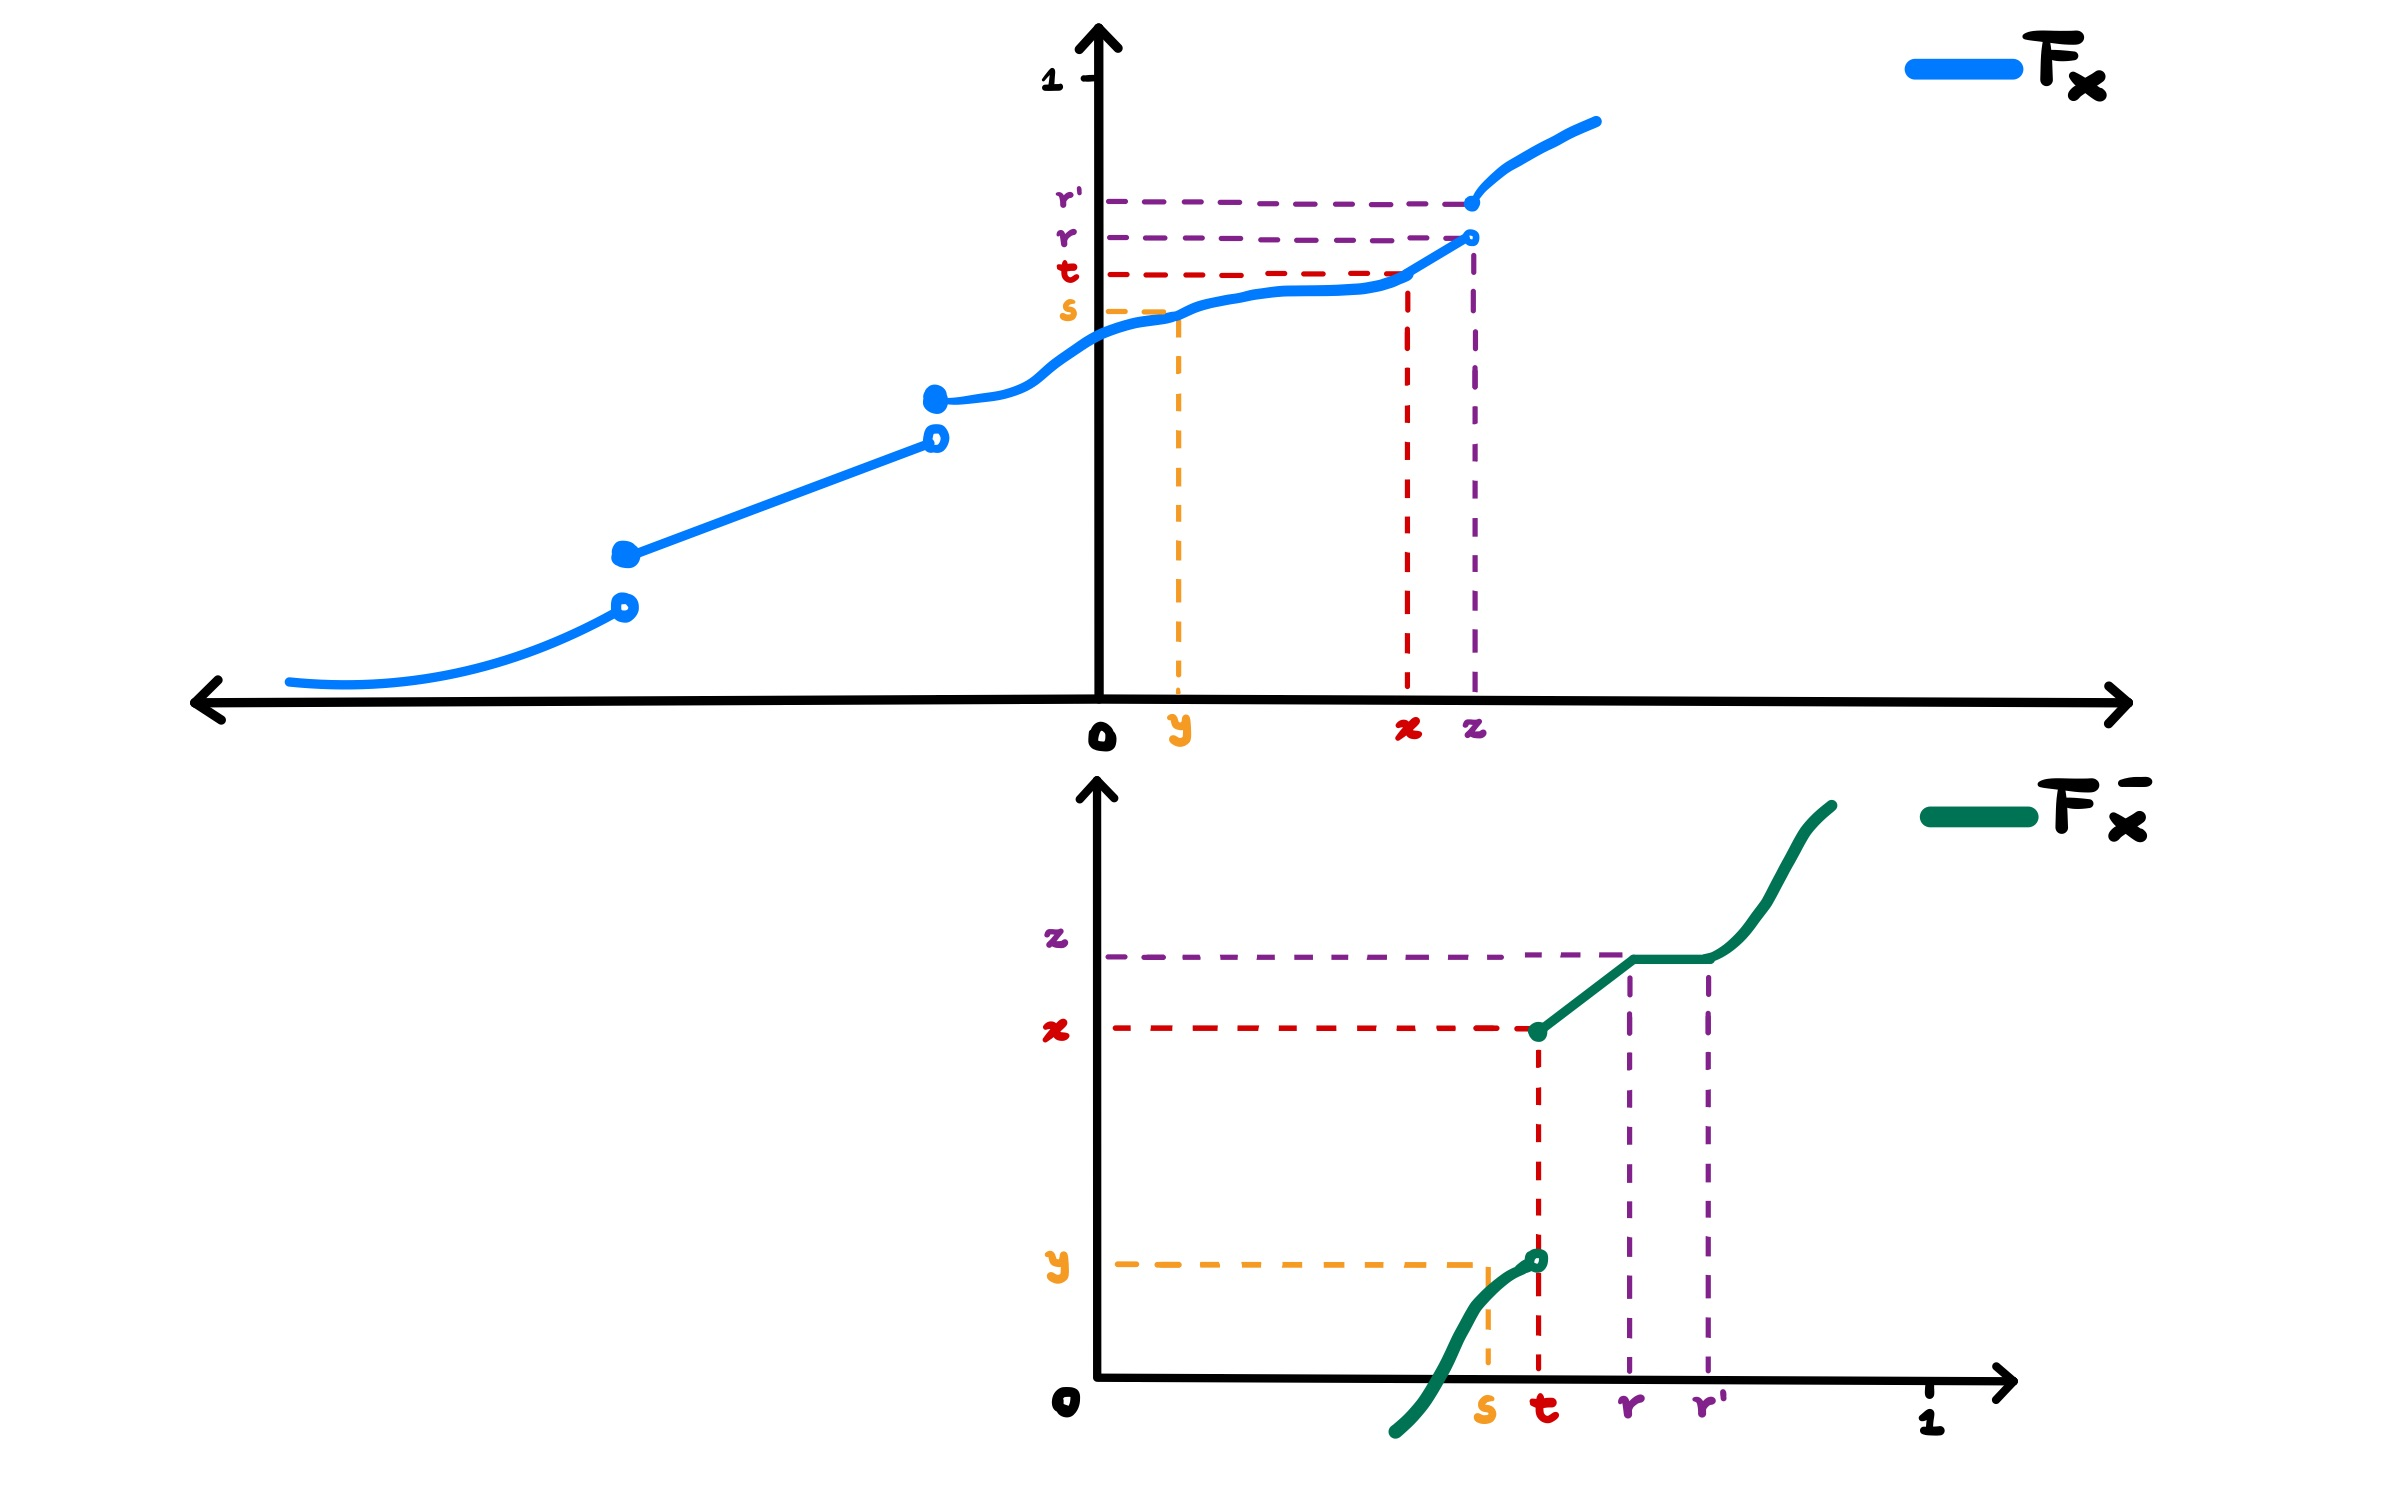
\includegraphics[scale=0.17]{img/clase_06_pag_10.jpg}
%     \caption{Ejemplo de inversa generalizada}
%     \label{fig:inv_gen}
% \end{figure}
\begin{images}[\label{fig:inv_gen}]{Ejemplo de inversa generalizada}
	\addimage{clase_06_pag_10_01}{width=11cm}{Función $F_X$}
	\imagesnewline
    \addimage{clase_06_pag_10_02}{width=10cm}{Función $F^-_{\mbox{ }X}$}
\end{images}

\vspace{1.5cm}\\
Veamos como se aplica el método de la inversa generalizada a las variables aleatorias \textbf{exponencial} y \textbf{Poisson}.

\begin{definition}[Variable exponencial]
Dado $\lambda>0$ la v.a. $X$ se dice exponencial si su densidad está dada por:
$$ f_X(x) = \lambda e^{-\lambda x}, \forall x\geq 0 \, ,$$
lo cual se denota $X\sim exp(\lambda)$.
\end{definition}

Sea la v.a. $X\sim exp(\lambda)$ con $\lambda>0$. Notemos que su función distribución está dada por \\ $F_X(x)=1-e^{-\lambda x}$. Luego por Proposición \ref{propinvgen},
$$\Finvgen(z)=\displaystyle\frac{-\ln(1-z)}{\lambda} \, .$$
Además, como tenemos $1-U\igualley U$, se sigue el siguiente corolario:
\begin{corolary}[Simulación de una exponencial con inversa generalizada]
\label{simexp}  %%
Sea la v.a. $X\sim exp(\lambda)$ con $\lambda>0$, entonces
% Sea la v.a. $X\sim exp(\lambda)$ con $\lambda>0$. Notemos que su función distribución está dada por \\ $F_X(x)=1-e^{-\lambda x}$. Luego por Proposición \ref{propinvgen}, 
$$X=\displaystyle\frac{-\ln(1-U)}{\lambda}\sim exp(\lambda) \, .$$
\end{corolary}

\begin{definition}[Distribución Poisson]
Dado $\lambda>0$ decimos que la v.a. $N$ posee distribución de Poisson de parámetro $\lambda$ si su función de distribución está dada por:
$$ \P(N=n)=\displaystyle\frac{e^{-\lambda}\lambda^n}{n!} \, .$$
\end{definition}
\begin{remark}
Recordemos que la distribución de Poisson aproxima el número de éxitos cuando repetimos muchas veces un experimento con probabilidad baja de éxito cada vez. Equivale al máximo $n\in\N$ tal que la suma de $n$ exponenciales no sume más que $\lambda$.
\end{remark}
Usando esto y el Corolario \ref{simexp} tenemos lo siguiente:
\begin{corolary}[Simulación de una Poisson con inversa generalizada]
Sean $(U_i)_{i\in\N} \, \iid$ y sea $\lambda>0$, entonces
$$ N = \sup\{n\in\N : \displaystyle - \sum^n_{i=1}\ln(U_i)<\lambda\}$$
% Sea $N$ distribución de Poisson, luego podemos simular $N$ como
tiene ley de Poisson de parámetro $\lambda$.
\end{corolary}
\subsubsection{Gaussianas}
Consideremos dos distribuciones Gaussianas independientes (ver definición \ref{gauss}). Para simularlas usaremos la transformada de Box-Muller:

\begin{proposition}[Método de Box-Muller] 
Sean $U,V\sim\unif$, definimos:
$$R:=\displaystyle\sqrt{-2 \ln U}\, ,$$ y $$ \hat{\theta}:=(cos(2\pi V),sen(2\pi V)) \, .$$
Luego tenemos
$$ X=(X_1,X_2):=R\hat{\theta}\sim\normal(0,I_2) \, .$$
O sea, $X_1\indep X_2$ y $X_1,X_2\sim\normal(0,1)$.
\end{proposition}
\begin{proof}
\ejercicio. \gris Indicación: usar teorema de cambio de variables en $\R^2$. \negro
\end{proof}

\subsubsection{Variables aleatorias discretas cualquiera}
\label{disc}
Queremos simular $X$ v.a. discreta que toma valores $x_1<x_2<x_3<\dots<x_n<\dots$ $n\in\N$.
\begin{proposition}
Sea $X$ v.a. discreta y $p_n=\P(X=x_n)$ su función de probabilidad. Definimos una partición de $[0,1]:0=a_0<a_1<\dots<a_n\leq1$ mediante $a_n=\sum_{k\leq n}p_k$. Entonces podemos simular $X$ usando
$$ Y:=\displaystyle\sum_{n\in\N}x_n \mathbf{1}_{a_{n-1},a_n}(U)\igualley X \, .$$
\end{proposition}
\begin{proof}
Basta ver que $Y=\Finvgen(U)$. \ejercicio
\end{proof}

\subsubsection{Caso inversa no explícita}
Sea $X$ variable aleatoria real con densidad $f_X$ estrictamente positiva. Entonces la función de distribución $F_X$ es derivable y estrictamente creciente. Si \textbf{no conocemos} $F_X$ %la inversa 
o no la podemos invertir, usaremos el siguiente método:
\begin{definition}[Aproximación de Newton-Raphson]
Dado $U\in[0,1]$ queremos encontrar el único $\bar{x}$ tal que $F_X(\bar{x})=U$ (de este modo $\bar{x}=\Finvgen(U)$). Es decir, buscamos la única raíz de $G(x)=F_X(x)-U$.
\newline Luego el método de Newton-Raphson consiste en tomar:
$$ x_n:=x_{n-1}-\displaystyle\frac{G(x_{n-1})}{G'(x_{n-1})}=x_{n-1}-\frac{(F_X(x_{n-1})-U)}{f_X(x_{n-1})}\conv \bar{x} \, ,$$
e iterar hasta que ($F_X(x_k)-U$)$\leq\delta$ para $\delta$ pequeño dado.
\end{definition}

\subsection{Método general}
\subsubsection{Aceptación-rechazo}
\label{metgen}
Supongamos que queremos simular v.a. $X$ en $E$ espacio medible, con densidad conocida $f$ con respecto a una medida $\lambda(dx)$ en $E$, y que existe $Y$ v.a. en $E$ con densidad $g$ con respecto a $\lambda$ tal que:
\begin{itemize}
    \item sabemos simular fácilmente $Y$
    \item $\exists K>0 \tq f(x)\leq Kg(x)\mbox{ } \forall x \tq g(x)>0$
\end{itemize}
Veremos a continuación que podemos simular $X$ usando una sucesión $\iid (Y_n,U_n)_{n\geq 1}$ con $Y_n\igualley Y$, $U_n\sim\unif$ y $Y_n\indep U_n$. La segunda condición nos dice que no es necesario que $g$ ``domine'' $f$, sin embargo lo haría si amplificamos por una constante $K$.
\newp Vamos a necesitar la función siguiente:  % , $\forall x \in E$, definimos
% $$ \alpha(x):=\displaystyle\frac{f(x)}{Kg(x)}\in[0,1] \, .$$ 
$$ \alpha(x) := \begin{cases} 
    \displaystyle\frac{f(x)}{Kg(x)}  & \mbox{ si }g(x)>0\\
    0 & \mbox{ si }g(x)\leq0  \, .
\end{cases}$$
% Notemos que si $g(x)>0$,  $\alpha(x)\in[0,1]$. %$\frac{f(x)}{Kg(x)}\in[0,1]$.
Notemos que $\alpha(x)\in[0,1]$. Además $\displaystyle\int f \lambda(dx)\leq K\int g\lambda(dx)$, luego $K\geq 1$.
% \newp Luego se tiene la siguiente proposición:
\begin{proposition}[Método de aceptación-rechazo]
Sea $E$ un espacio medible cualquiera. Consideramos $X$ v.a. en $E$ con densidad $f$ e $Y$ v.a. en $E$ con densidad $g$ de modo que $\exists K>0 \tq $
$$f(x)\leq Kg(x) \espacio \forall x\in \{z\in E \,|\,g(z)>0 \}$$
\newline Sea $N=\inf\{n\geq 1:U_n\leq \alpha(Y_n)\}$, entonces tenemos:
\begin{itemize}
    \item[(i)] $N\sim Geom(\frac{1}{K})$
    \item[(ii)] $Y_N\sim Ley(X)$
    \item[(iii)] $Y_N\indep N$
\end{itemize}
\end{proposition}
\begin{proof}
\gris 
\begin{alignat*}{2}
    \P(Y_N\in A, N=m) & = \P(Y_m\in A, U_m \leq \alpha(Y_m),U_k>\alpha(Y_k),k=1,\dots,m-1) \\
     & = \P(Y_m\in A,U_m\leq \alpha(Y_m))(1-p)^{m-1} %\, .
     % \\ & = \displaystyle \int_A(\int^{\alpha(y)}_0 dt)g(y)\lambda(dy)(1-p)^{m-1}
     \\&  = \displaystyle \int_A \left(\int^{\alpha(y)}_0 dt\right)g(y)\lambda(dy)(1-p)^{m-1}
     \\ & = \frac{1}{K}\int_Af(y)\lambda(dy)(1-p)^{m-1} \, ,
\end{alignat*}
donde $p=\P(U_1\leq\alpha(Y_1))$. Luego tomando $A=E$ obtenemos
\begin{alignat*}{2}
    \P(N=m) & = \P(U_m \leq \alpha(Y_m))(1-p)^{m-1} \\
     & = p(1-p)^{m-1}
     \\ & = \frac{1}{K}(1-p)^{m-1} \, .
\end{alignat*}
Luego $p=\P(U_m\leq \alpha(Y_m))=\frac{1}{K}$, y $\therefore \espacio N\sim Geom(p)=\frac{1}{K}$.
\\ Así,
\begin{alignat*}{2}
    \P(Y_N\in A, N=m) & = \displaystyle \int_A f(y)\lambda(dy) p(1-p)^{m-1} \\
     & = \P(X\in A)p(1-p)^{m-1}
     \\ & =  \P(X\in A)\P(N=m) \, .
\end{alignat*} 
Sumando sobre $m\geq 1$ nos queda que
$$ \P(Y_N\in A) = \P(N=m)$$
Por ende $Y_n \igualley x$.
\\ Finalmente,
$$ \P(Y_N\in A, N=m) = \P(Y_N\in A)\P(N=m) $$
$\therefore \espacio Y_N\indep N$
\findem \negro
\end{proof}
% \vspace{.5cm}
\begin{remark}
\beforeitemize
\begin{itemize}
    \item Para obtener una realización de una v.a. de $Ley(X)$ se requiere simular una cantidad $N$ finita, pero aleatoria $\sim Geom(\frac{1}{K})$ (desconocida a priori) de pares $(Y_1,U_1),\dots,(Y_n,U_n),\dots$.
    \newline De ahí el nombre del método aceptación rechazo, pues si se cumple la condición aceptamos y si no rechazamos.
    \item $N\sim Geom(\frac{1}{k}) \implies \E(N)=K$. Luego, mientras más pequeño sea $K\geq 1$ tal que $f(x)\leq Kg(x)$, mejor, pues aceptamos el valor $Y_m$ más pronto.
    \item $K$ pequeño significa que g está más ajustada a $f$. Idealmente nos gustaría $K=1$, pero en ese caso tendríamos $0\leq g(x)-f(x)\implies 0\leq\int|g-f|\lambda(dx)=1-1=0\implies g\equiv f$ o sea, $X\igualley Y$. Si tuviésemos esto entonces ``ya sabríamos simular $X$'' ($Y$ es una v.a. que sabemos simular fácilmente).
\end{itemize}
\end{remark}

\subsubsection{Simulación condicional a subconjunto}
Como aplicación tenemos el siguiente corolario, donde \textbf{no necesitamos simular las uniformes}:
\begin{corolary}[Simulación de una v.a. $Y$  ``condicional a que $Y\in A$'']
\label{corclase7}
\newline Sean $(Y_n)_{n\geq 1}$ réplicas $\iid$ (simulables) de una v.a. $Y$ en $E$ y $A\subset E$. Sea $N:=\inf\{n\geq 1: Y_n\in A\}$, entonces
$$ \hat{Y}:=Y_N\sim Ley(Y|Y\in A) \espacio \mbox{ y }\espacio Y_N\indep N \, .$$
\end{corolary}
\begin{proof}
\gris
$X\sim Ley(Y|Y\in A)$ tiene densidad $f$ con respecto a $\lamnda=Ley(Y)$, dada por
$$ f(x) = K\mathbf{1}_A(x) = \P(Y\in A)^{-1}\mathbf{1}_A(x)\leq K g(x) \, ,$$
con $g\equiv 1$ la densidad $Y$ con respecto a $\lambda$.  Por el método aceptación-rechazo, $Y_N\sim Ley(Y|Y\in A)$, para $N=\inf\{n\geq1:U_n\leq\alpha(Y_n)\}$, donde $(U_n)_{n\in\N}\indep (Y_n)_{n\geq1}$ son $\iid$ y distribuyen $\unif$. Pero $U_n\leq\alpha(Y_n)=\mathbf{1}_A(Y_n)\Longleftrightarrow Y_n\in A$
\findem
\negro
\end{proof}

% \begin{proposition}[Caso particular de Corolario \ref{corclase7}]
\subsection{Variables condicionadas a estar en un intervalo}
\begin{proposition}
Consideramos $X$ una v.a. real cualquiera y $A=[a,b]$. Sea $V\sim\mathbb{U}([F_X(a),F_X(b)])$.
Notemos que 
$$V\igualley F_X(a)+U(F_X(b)-F_X(a))$$
con $U\sim \unif$. Entonces
$$ \Finvgen (V) \sim Ley(x \, |\, x\in[a,b]) \, .$$
\end{proposition}
\begin{proof}
\ejercicio
\newline \gris Indicación: demostrar y utilizar: $F_{\{x|x\in[a,b]\}}(x)=\displaystyle\frac{F_X(x)-F_X(a)}{F_X(b)-F_X(a)}$. \negro
\end{proof}
% \vspace{1cm}
\subsection{Técnicas de reducción de varianza en M.M.C}
Para una presentación sucinta de estos temas ver el capítulo 1 del libro \textit{Processus de Markov et applications. Algorithmes, Réseaux, Génome et
Finance}, capítulo 1, É. Pardoux \cite{pardoux} y con el algo más de profundidad \textit{Monte -Carlo methods in financial engineering} de P. Glasserman, capítulo 1. Para más detalles ver Asmussen ``Stochastic Simulation'' \cite{asm}.
\newp \textbf{Idea}: si disponemos de $Y_1,\dots,Y_n,\dots \iid$ para aproximar $I=\E(Y)$, el error cometido será menor si $\sigma^2=\var(Y)$ es menor (para igual $\E(Y)$).
\begin{itemize}
    \item $\E(|\bar{Y}_n-I|^2)=\displaystyle\frac{\var(Y)}{n}$
    \item con un nivel de confianza $\alpha\in(0,1)$ dado, $\P(|\bar{Y}_n-I|<\epsilon)\gtrsim 1-\alpha$ si $n\geq\nmc$
\end{itemize}
Luego si podemos simular $Y'_1,\dots,Y'_n$ tal que $\E(Y')=I$ y $\var(Y')<\var(Y)$ (a costo comparable), necesitaremos menos ``$n$''s y seremos más eficientes.
\newp Los métodos de reducción de varianza que veremos son los siguientes:
\begin{enumerate}
    \item Variable de control (\ref{control})
    \item Variables antitéticas (\ref{antitéticas})
    \item Muestreo preferencial (\ref{preferencial})
    \item Muestreo estratificado (\ref{estratificado})
\end{enumerate}
Notar de todos modos que para comparar dos métodos de calcular $I=\E(Y)$, de todas maneras hay que considerar el costo ``por réplica''.

\subsubsection{Variable de Control}
\label{control}
Supongamos que podemos simular $Y=f(X)$ y que conocemos $\E(h(X))$ explícitamente para cierta función real $h$, que llamaremos  \textbf{variable de control}.
\newp Disponemos entonces de muchos ``estimadores'' de $I$ ``posibles'': para cada $c\in\R$,
$$ \sumfx+c\mbox{ }[\frac{1}{n}\sum_{k=1}h(X_k)-\E(h(X))] 
 =\frac{1}{n}\sum_{k=1}^n[f(X_k)+c(h(X_k)-\E(h(X))]
 =\frac{1}{n}\sum^n_{k=1}\varphi_c(X_k) \, ,$$
con $\E(\varphi_c(X_1))=I$.\hspace{.3cm} ¿Cual es su varianza?
\begin{alignat*}{2}
    \var(\varphi_c(X_1)) & = \var(f(X_1)+ch(X_1)) \\
     & = \var(f(X_1))+c^2\var(h(X_1))+2\mbox{ }c\mbox{ }Cov(h(X_1),f(X_1)) \, .
\end{alignat*}
% $$ \var(\varphi_c(X_1))=\var(f(X_1)+ch(X_1)) = \var(f(X_1))+c^2\var(h(X_1))+2\mbox{ }c\mbox{ }Cov(h(X_1),F(X_1))$$
De lo anterior se desprende que la varianza disminuye cuando se cumple:
$$ c^2 Var(h(X)) + 2c Cov(h(X),f(X)) < 0 $$

Además podemos optimizar en $c\in\R$. Queda:
$$ c^*=\displaystyle\frac{-Cov(f(X_1),h(X_1))}{\var(h(X_1))} \, .$$
%i.e., hacemos que los dos términos finales se cancelen. Así quedará sólo la varianza de $f(X_1)$. 
Substituyendo arriba:
$$ \var(\varphi_{c^*}(X_1))=\sigma^2-\displaystyle\frac{Cov(f(X_1,h(X_1)))^2}{\var(h(X_1))} \, .$$
Luego $\var(\varphi_{c^*}(X_1))<\sigma^2$ si $Cov(f(X_1,h(X_1))\neq 0$, i.e., reducimos la varianza del estimador.
\newp En general, quizás no conocemos $Cov(f(X_1,h(X_1))$ ni $\var(h(X_1))$. Pero los podemos estimar con $q$ (pequeño) simulaciones ``piloto''. Primero, usando la Ley de grandes números tenemos que,
$$ \displaystyle\frac{\sum_{k=1}^q(Y_k-\bar{Y}_q)(Z_k-\E(Z_1))}{q-1} \mbox{ }\substack{\longrightarrow \\ q\to\infty}\mbox{ } Cov(Y_1,Z_1) \, ,$$
entonces
$$ Cov(f(X_1,h(X_1)))\approx \displaystyle\frac{\sum_{k=1}^q(Y_k-\bar{Y}_q)(Z_k-\E(Z_1))}{q-1} \, ,$$
con $Y_k=f(X_k),Z_k=h(X_k)$ y 
$$\var(h(X_1))\approx \displaystyle\frac{\sum_{k=1}^q(Z_k-\E(Z_k))^2}{q-1} \, ,$$
luego,
$$ \hat{c}^*=\displaystyle\frac{\sum_{k=1}^q(Y_k-\bar{Y}_q)(Z_k-\E(Z_1))}{\sum_{k=1}^q(Z_k-\E(Z_k))^2} \, ,$$
y aproximaremos entonces $I$ mediante el siguiente promedio empírico:
$$ \displaystyle \frac{1}{n}\sum^q_{k=1}[f(X_k)-\hat{c}^*(h(X_k))-\E(h(X_1))]=\frac{1}{n}\sum^q_{k=1}\hat{\varphi}(X_k) \, .$$
\begin{example}[Ejemplo ``juguete'' de aplicación de variable de control]
Queremos calcular $I=\int^1_0e^xdx$ (ya sabemos que esto vale $e-1$).
\newp Método ``usual'': $I=\E(f(X))=\E(e^X),X\sim \unif$ donde $\var=\var(e^X)\approx0,242$
\newp Por otro lado, considerando $h(X_1)=\int^1_0(x+1)dx$ como variable de control:
$$ I=\int^1_0e^xdx - (\int^1_0(x+1)dx-\frac{3}{2})=\int^1_0(e^x-1-x)dx+\frac{3}{2} \, .$$
Tomando $c=-1,h(X)=x+1$. En este caso se puede verificar que:
$$ \var(e^X-1-x)\approx0.00437 \, .$$
Esto es 5 veces menos que $Var(e^X)$.
\end{example}

\subsubsection{Variables antitéticas (de a pares)}
\label{antitéticas}
Sea $I=\E(Y)$ con \hspace{.2cm} $Y=f(X)$ y \hspace{.2cm} $X$ v.a. en $\R$. Consideremos el M.M.C usual usando $(X_n)_{n\geq1}\iid \sim Ley(x)$, con $\var(f(x))=\sigma^2$. Para un número par $2n$ de réplicas $Y_k=f(X_k)$, $\bar{Y}_{2n}=\frac{1}{2n}(Y_1+\dots+Y_{2n})\conv I$ con $ECM_{2m}=\E(|\bar{Y}_{2n}-I|^2)=\displaystyle\frac{\sigma^2}{2n}$ (error cuadrático medio).
\newp Supongamos que simultáneamente podemos simular $(X_n')_{n\geq 1}\sim Ley(X)$ de modo que $X_n$ y $X_n'$ están \textbf{correlacionadas}, y la sucesión de pares $(X_n,X_n')_{n\geq1}$ son $\iid$ (independiente de los anteriores). Entonces también:
$$ \displaystyle\frac{1}{2}(\bar{Y}_n+\bar{Y}_n')=\frac{1}{2n}[(Y_1+Y_1')+\dots+(Y_n+Y_n')]\conv I\, .$$
\textbf{¿Con qué $ECM'_{2m}$?}
\newline $\displaystyle\frac{1}{2}(\bar{Y}_n+\bar{Y}_n')=\frac{1}{n}\sum^n_{k=1}\frac{(Y_k+Y_k')}{2}$ con $\frac{Y_k+Y_k'}{2}=\frac{f(X_k)+f(X_k')}{2},\mbox{ } k\geq1\mbox{ }\iid$ de media $\E(f(X))=I$.
\begin{alignat*}{2}
ECM_2n' & = \E\bigg(\bigg|\frac{1}{2}(\bar{Y}_n+\bar{Y}_n'-I)\bigg|^2\bigg) \\
& =\frac{1}{n}\var\bigg(\frac{Y_1+Y_1'}{2}\bigg) \\
& =\frac{1}{4n}[2\var(Y_1)+2\cov(Y_1,Y_1')] \\
& =\frac{1}{2n}(\sigma^2+\cov(f(X_1),f(X_1')))
\end{alignat*}
% $$ECM_2n'=\E(|\frac{1}{2}(\bar{Y}_n+\bar{Y}_n'-I)|^2)=\frac{1}{n}\var(\frac{Y_1+Y_1'}{2})=\frac{1}{4n}[2\var(Y_1)+2\cov(Y_1,Y_1')]=\frac{1}{2n}(\sigma^2+\cov(f(X_1),f(X_1')))$$
Luego si $\cov(f(X_1),f(X_1'))<0$, $$ECM'_{2n}<\frac{\sigma^2}{2n}=ECM_{2n} \, .$$
Aplicación usual: $X_n=U_n\sim\unif$, $X_n'=1-U_n\sim\unif$ (la realización $U_n$ es la misma para $X$ y $X'$), y las $2n$ variables aleatorias $U_1,\dots,U_n$, $1-U_1,\dots1-U_n$ requieren solo $n$ simulaciones.
\newp \textbf{¿Cuando se tiene $\cov(f(U_1),f(1-U_1))\leq 0$?}
Respondemos esto con el siguiente lema.
\begin{lemma}
Sea $f:[0,1]\to\R$ función monótona tal que $f\in L^2([0,1],dx)$. Entonces $\cov(f(U),f(1-U))\leq0$.
\end{lemma}
\begin{proof}  % 10:40
\gris
Sea $\tilde{U}\sim \unif$, $\tilde{U}\indep U$. Para $f$ creciente o decreciente siempre tenemos
$$ (f(U)-f(\tilde{U}))(f(1-U)-f(1-\tilde{U})) \leq 0 \, .$$
Tomando la esperanza se tiene que
$$ 2(\E(f(U)f(1-U))-\E(f(U))\E(f(1-\tilde{U})))\leq 0 $$
$$ \Longleftrightarrow \E(f(U)f(1-U))-\E(f(U))^2 \leq 0 \, .$$
\findem
\negro
\end{proof}

\textbf{Receta general}: Luego si tenemos $f:[0,1]\to\R$ monótona (por ejemplo $f=F^-_{\mbox{ }Z}$ una función de distribución inversa) usando $n$ réplicas $\unif$, el estimador: $$\displaystyle\frac{1}{n}\sum^n_{k=1}[\frac{f(U_k)+f(1-U_k)}{2}]$$ aproxima $I=\E(f(U))$ con varianza menor a $\sigma^2/2n$, es decir, menos de la mitad de la varianza $\sigma^2/n$ del estimador usual: $$\displaystyle\frac{1}{n}\sum^n_{k=1}f(U_k)$$ construido con las mismas $n$ réplicas.
%\textbf{Receta general}: cuando tengamos $f$ función monótona aplicada a una uniforme $U$, entonces en vez de usar
%$$\displaystyle\frac{1}{n}\sum^n_{k=1}f(U_k)$$
%Usamos $$\displaystyle\frac{1}{n}\sum^n_{k=1}[\frac{f(U_k)+f(1-U_k)}{2}] $$
%Y reduciremos la varianza a la mitad.
\vspace{1cm}\\
\subsubsection{Muestreo preferencial (\textit{importance sampling})}
\label{preferencial}
Queremos calcular $I=\E(f(X))=\int f(x)\mu(dx)$ con $X\sim \mu$ y supongamos que podemos simular $Z\sim\nu$ simulable tal que $\nu\approx\mu$ .  % con $Z\sim \nu$ simulable. 
Es decir $\exists L:\R^d\to\R_+$ densidad de Radon-Nikodym tal que $\nu(dx)=L(x)\mu(dx)$ con $L>0$ $\mu-c.s.$,
\newline Entonces 
$$I=\displaystyle\int\frac{f(x)}{L(x)}\nu(dx)\, ,$$ 
y podemos calcular $I$ también como 
$$I=\displaystyle\E\left(\frac{f(Z)}{L(Z)}\right) \, .$$
\textbf{¿Podemos encontrar $\nu$ así, de manera que además $\var(\frac{f(Z)}{L(Z)})<\var(f(X))$?}
\begin{remark}
\begin{alignat*}{2}
    \var\left(\displaystyle\left(\frac{f(Z)}{L(Z)}\right)\right) & = \E\left(\frac{f(Z)^2}{L(Z)^2}\right)-I^2\\
     & = \int \frac{f(z)^2}{L(z)^2}\mu(dz) - [\int f(x)\mu(dx)]^2 \\
     & = \int \frac{|f(z)|}{L(z)}\frac{|f(z)|}{L(z)}\mu(dz) - [\int f(x)\mu(dx)]^2 \\
     & = \int |f(z)|\frac{|f(z)|}{L(z)}\mu(dz) - [\int f(x)\mu(dx)]^2 \, .
\end{alignat*}
\end{remark}
Si $f\geq0$, tomando $L(z)=\displaystyle\frac{f(Z)}{I}$, o sea $\nu(dz)=\displaystyle\frac{f(Z)}{I}\mu(dz)$ y obtendríamos 
$$\var\left(\frac{f(Z)}{L(Z)}\right)=0 \, ,$$
pues $\frac{f(Z)}{L(Z)}=I$.
% \begin{remark}
\newp Lo anterior no se puede usar en la práctica porque \textbf{no conocíamos $I$}. Pero la fórmula $\nu(dz)=\frac{f(Z)}{I}\mu(dz)$ nos sugiere que sirve samplear de una ley parecida a $\mu$ (y equivalente) pero que da más peso a puntos $z$ tales que $f(z)$ es más grande, o sea que son \textbf{más importantes} en el cálculo de $\int f(x)\mu(dx)$.
% \end{remark}
\newp \textbf{Heurística}:
\begin{itemize}
    \item Buscar una medida $\tilde{\nu}$ ``parecida a $|f(x)|\mu(dx)$''
    \item Esta medida debe cumplir que $\nu(dx):=\displaystyle\frac{\tilde\nu(dx)}{\int\tilde{\nu}(dx)}$, sea ``\textbf{fácilmente simulable}'' donde $\int\tilde{\nu}(dx)$ es una constante de normalización calculable. 
\end{itemize}
\begin{example}[Aplicación ``artificial'' de muestreo preferencial]
Queremos aproximar $$I=\displaystyle\int^1_0\cos(\frac{\pi x}{2})dx=\frac{2}{\pi} \, ,$$ con $\mu(dx)=dx$ uniforme en $[0,1]$, $f(x)=\cos(\frac{\pi x}{2})$.\\
\newline Elegimos $\nu(dz)=\frac{z}{2}(1-z^2)dz=L(z)dz$ y aproximamos
$$ I\approx\displaystyle\frac{1}{n}\sum^n_{k=1}\cos(\frac{\pi z_k}{2})/L(z_k), \espacio Z_k \iid \sim \nu \, .$$
En la figura \ref{fig:pref} se grafican ambas funciones. Se puede mostrar que la varianza se reduce en factor mayor que $10$.
\begin{figure}
    \centering
    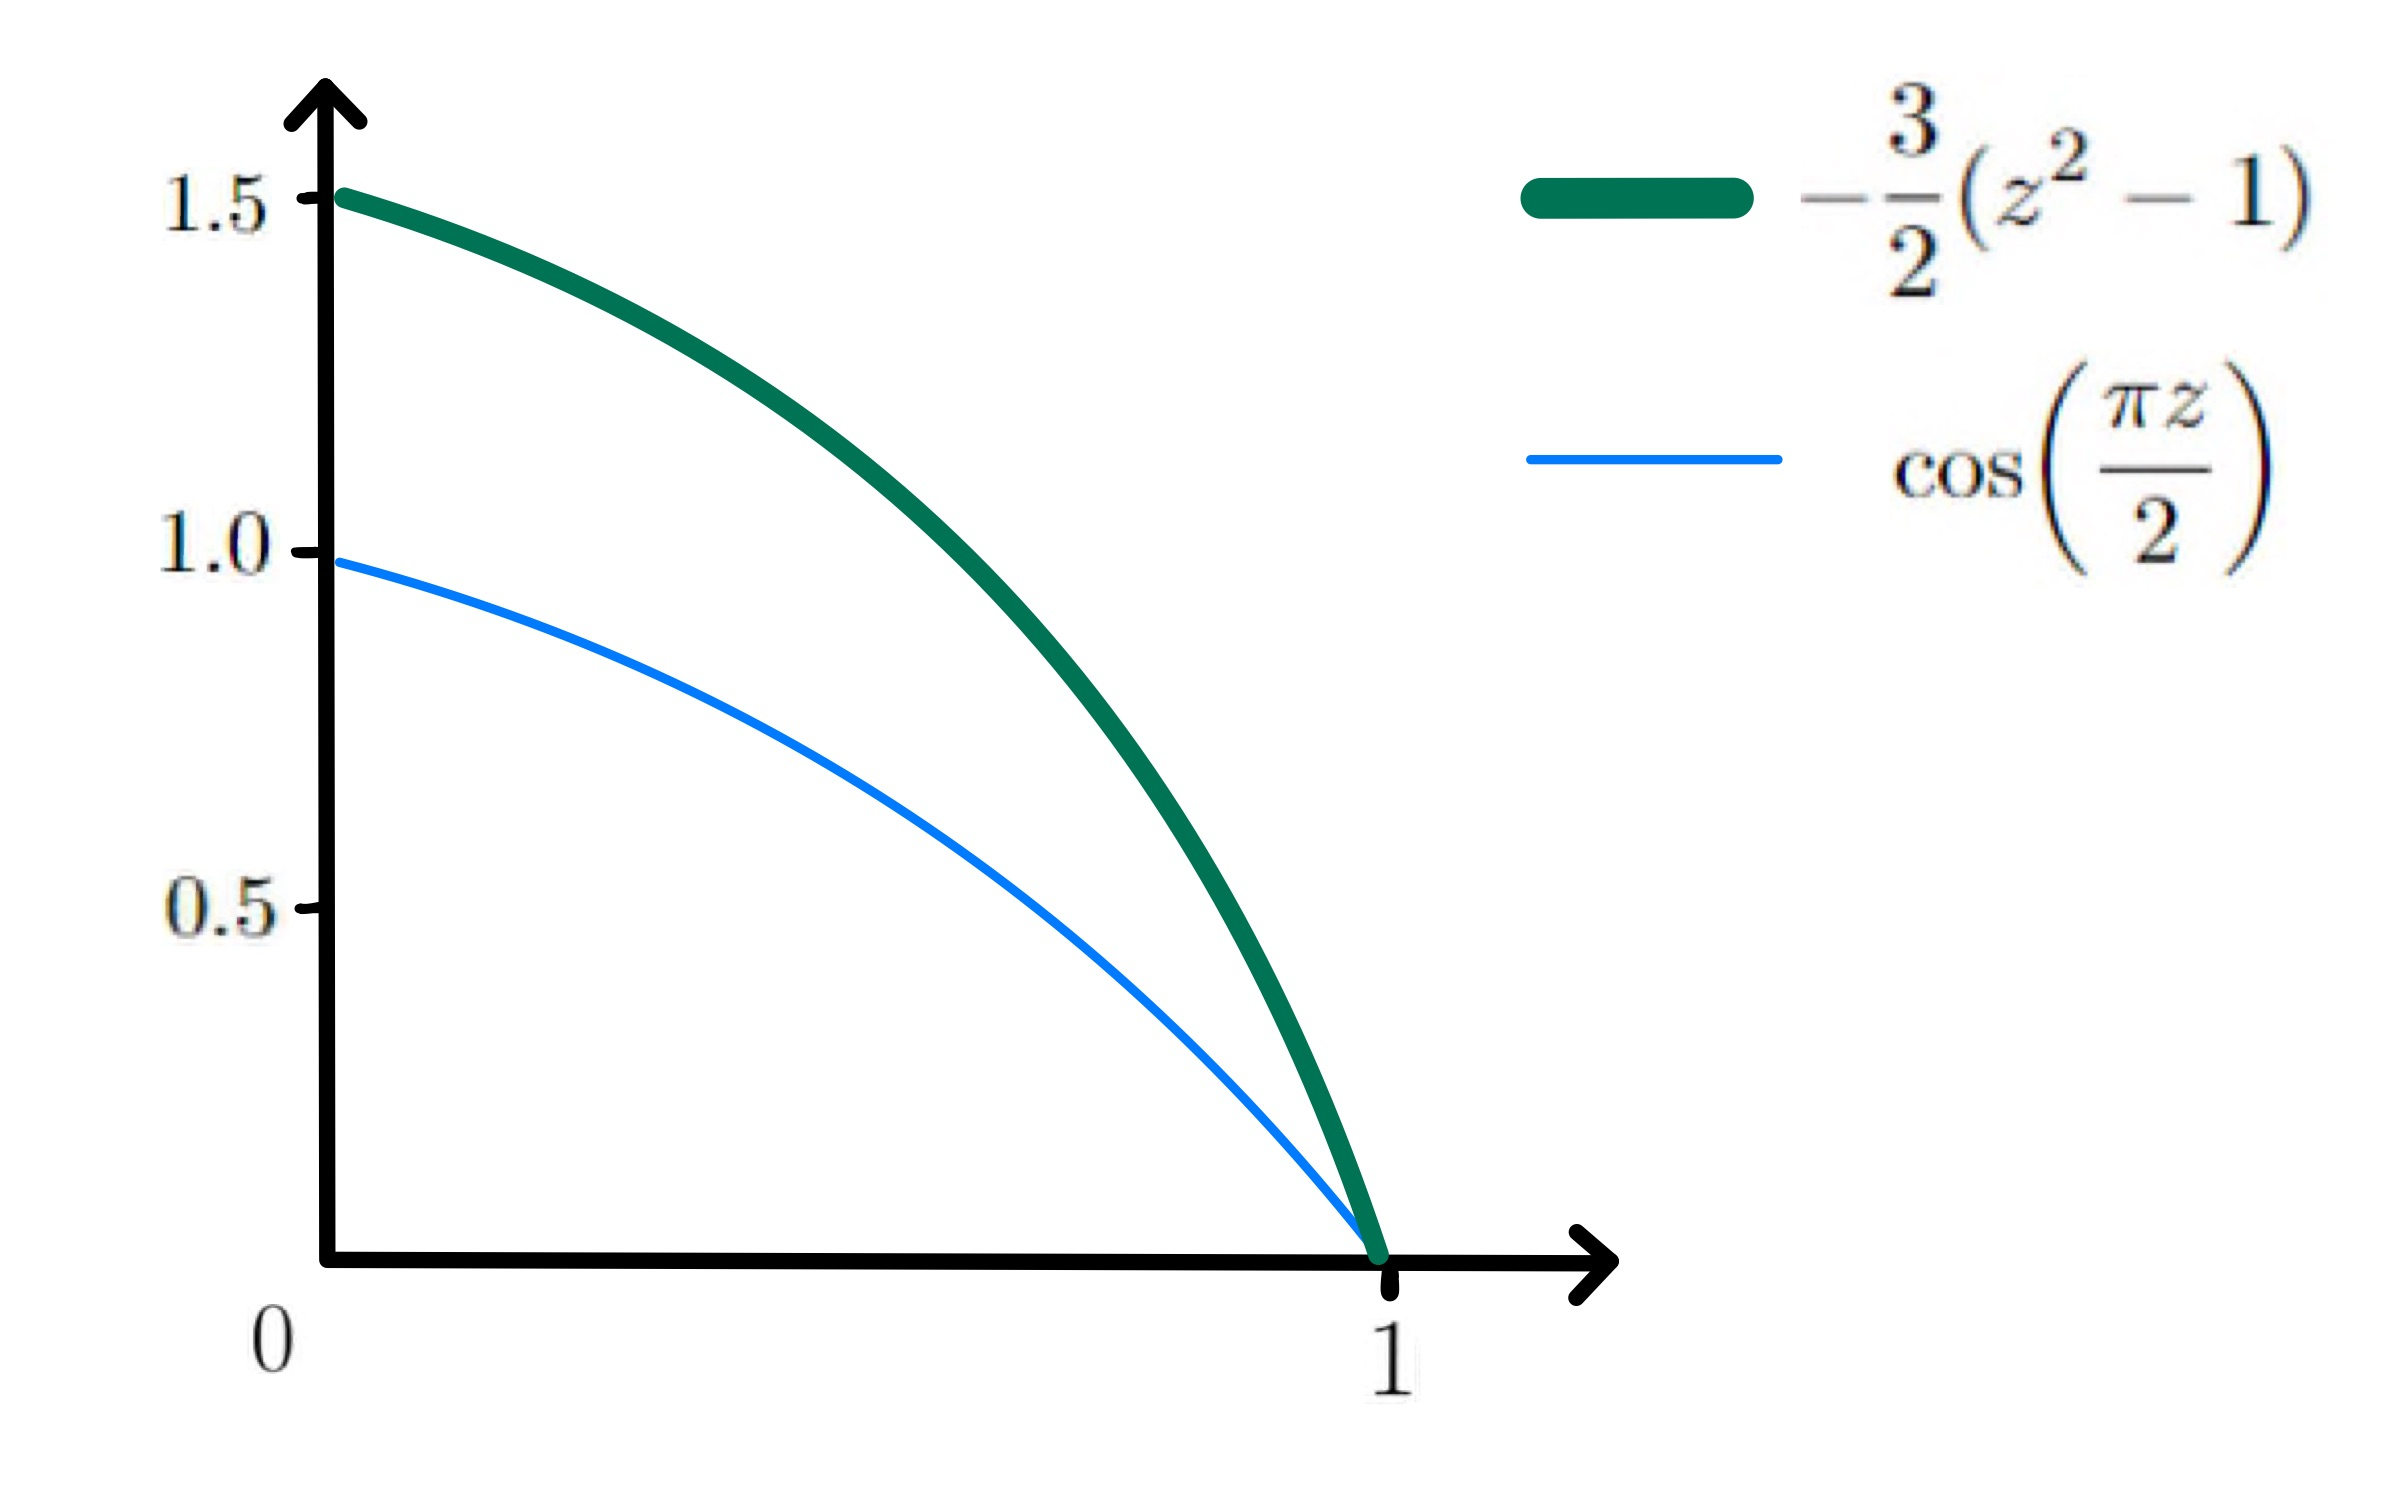
\includegraphics[scale=0.11]{img/clase_08_pag_11.jpg}
    \caption{Ejemplo de muestreo preferencial}
    \label{fig:pref}
\end{figure}
% \begin{images}[\label{fig:pref}]{Ejemplo de muestreo preferencial}
%     \addimage{clase_08_pag_11}{width=10cm}{}
% \end{images}
\end{example}

\subsubsection{Muestreo estratificado (\textit{stratified sampling})}
\label{estratificado}
Queremos calucular $I=\E(Y), Y$ v.a. $\in\R$ con $\sigma^2=\var(Y)$. 
\newline Supongamos que tenemos una partición $\mathcal{D}=\{D_1,\dots,D_k\}$ (``estratos'') de $\R$, conocemos \\ $p_i=\P(Y\in D_i)$, y sabemos simular $Y^j\sim Ley(Y | Y \in D_j)$ para cada $j=1,\dots,k$.
\begin{example}
En $\R$, $D_j$ de la forma $[a_j,b_j)$, vimos como simular $Y^j$ usando $F_Y^-$ y una v.a. $U[f_Y(a_j),f_X(b_j)]$.
\end{example}
Disponemos entonces de:
$$ n=n_1+\dots+n_k \mbox{ v.a. independientes }:\begin{cases}
Y^1_1,\dots,Y^1_{n_1} \iid \igualley Y^1 &\\
\dots & \\
Y^k_1,\dots,Y^k_{n_k} \iid \igualley Y^k &
\end{cases} $$
\textbf{¿Podemos estimar $I$ con $\var<\displaystyle\frac{\sigma^2}{n}=\var\left(\frac{1}{n}\sum^k_{j=1}Y_j\right)$ con $(Y_n)\igualley Y \iid$?}
Para responder a esto notemos que
\begin{alignat*}{2}
    \E(Y) & = \E(\E(Y|K)) \mbox{ con }K=j \mbox{ ssi }Y\in D_j\\
     & = \displaystyle\E(\sum^k_{j=1}\E(Y|K=j)\mathbf{1}_{k=j}) \\
     & = \displaystyle\sum^k_{j=1}p_j\E(Y^j) \, .
\end{alignat*}
Definimos
$$ \hat{Y}_n=\displaystyle\sum^k_{j=1}p_j\frac{1}{n_j}\sum^{n_j}_{i=1}Y^j_i \, .$$
\begin{remark}
\beforeitemize
\begin{itemize}
    \item $\E(\hat{Y}_n)=I$, es decir, $\hat{Y}_n$ que es un estimador insesgado de $I$.
    \item $\hat{Y}_n\to I$ c.s.  cuando  $n_1, \dots, n_k\to \infty $ con   $n=n_1+ \dots + n_k $, por Ley de Grandes N\'umeros. 
\end{itemize}
\end{remark}
% \begin{proof}
% \gris Probar que son insesgados y usar ley de grandes números en cada estrato. (\ejercicio)\negro
%\end{proof}
\textbf{¿Con qué ECM (varianza)?}
\newline Usando la independencia de las v.a.  $Y_{k}^j$,  tenemos: % En general:
$$ \var(\hat{Y}_n)=\displaystyle\frac{1}{n}\sum^k_{j=1}\frac{p_j^2}{n_j}\sigma^2_j \, .$$
Veamos que esto es menor que $\sigma^2/n$ \, . Usaremos la
\begin{proposition}[Fórmula de la ``varianza total'']
Sea $Y$ v.a. real y $K$ v.a. cualquiera, luego
$$ \var(Y)=\E(\var(Y|K))+\var(\E(Y|K)) \, .$$
Donde $\E(\var(Y|K))=\E((Y-\E(Y|K))^2|K)$.
\end{proposition}
\begin{proof}
\ejercicio
\end{proof}
Entonces aplicando lo anterior a  la v.a. $K$ definida como $K=j$ cuando $Y\in D_j$, obtenemos:
$$ \sigma^2\,=\,\displaystyle\sum^k_{j=1}p_j\sigma^2_j+\sum^k_{j=1}p_j(\E(Y^j)-\E(Y))^2\,\geq \,\sum^k_{j=1}p_j\sigma^2_j \, .$$
Aqu\'i, por un lado $\sum^k_{j=1}p_j\sigma^2_j$ corresponde a la esperanza de la varianza condicional, mientras que el término $\sum^k_{j=1}p_j(\E(Y^j)-\E(Y))^2$ es la varianza de la esperanza condicional (ver Figura \ref{fig:estrat}). 
\begin{figure}
    \centering
    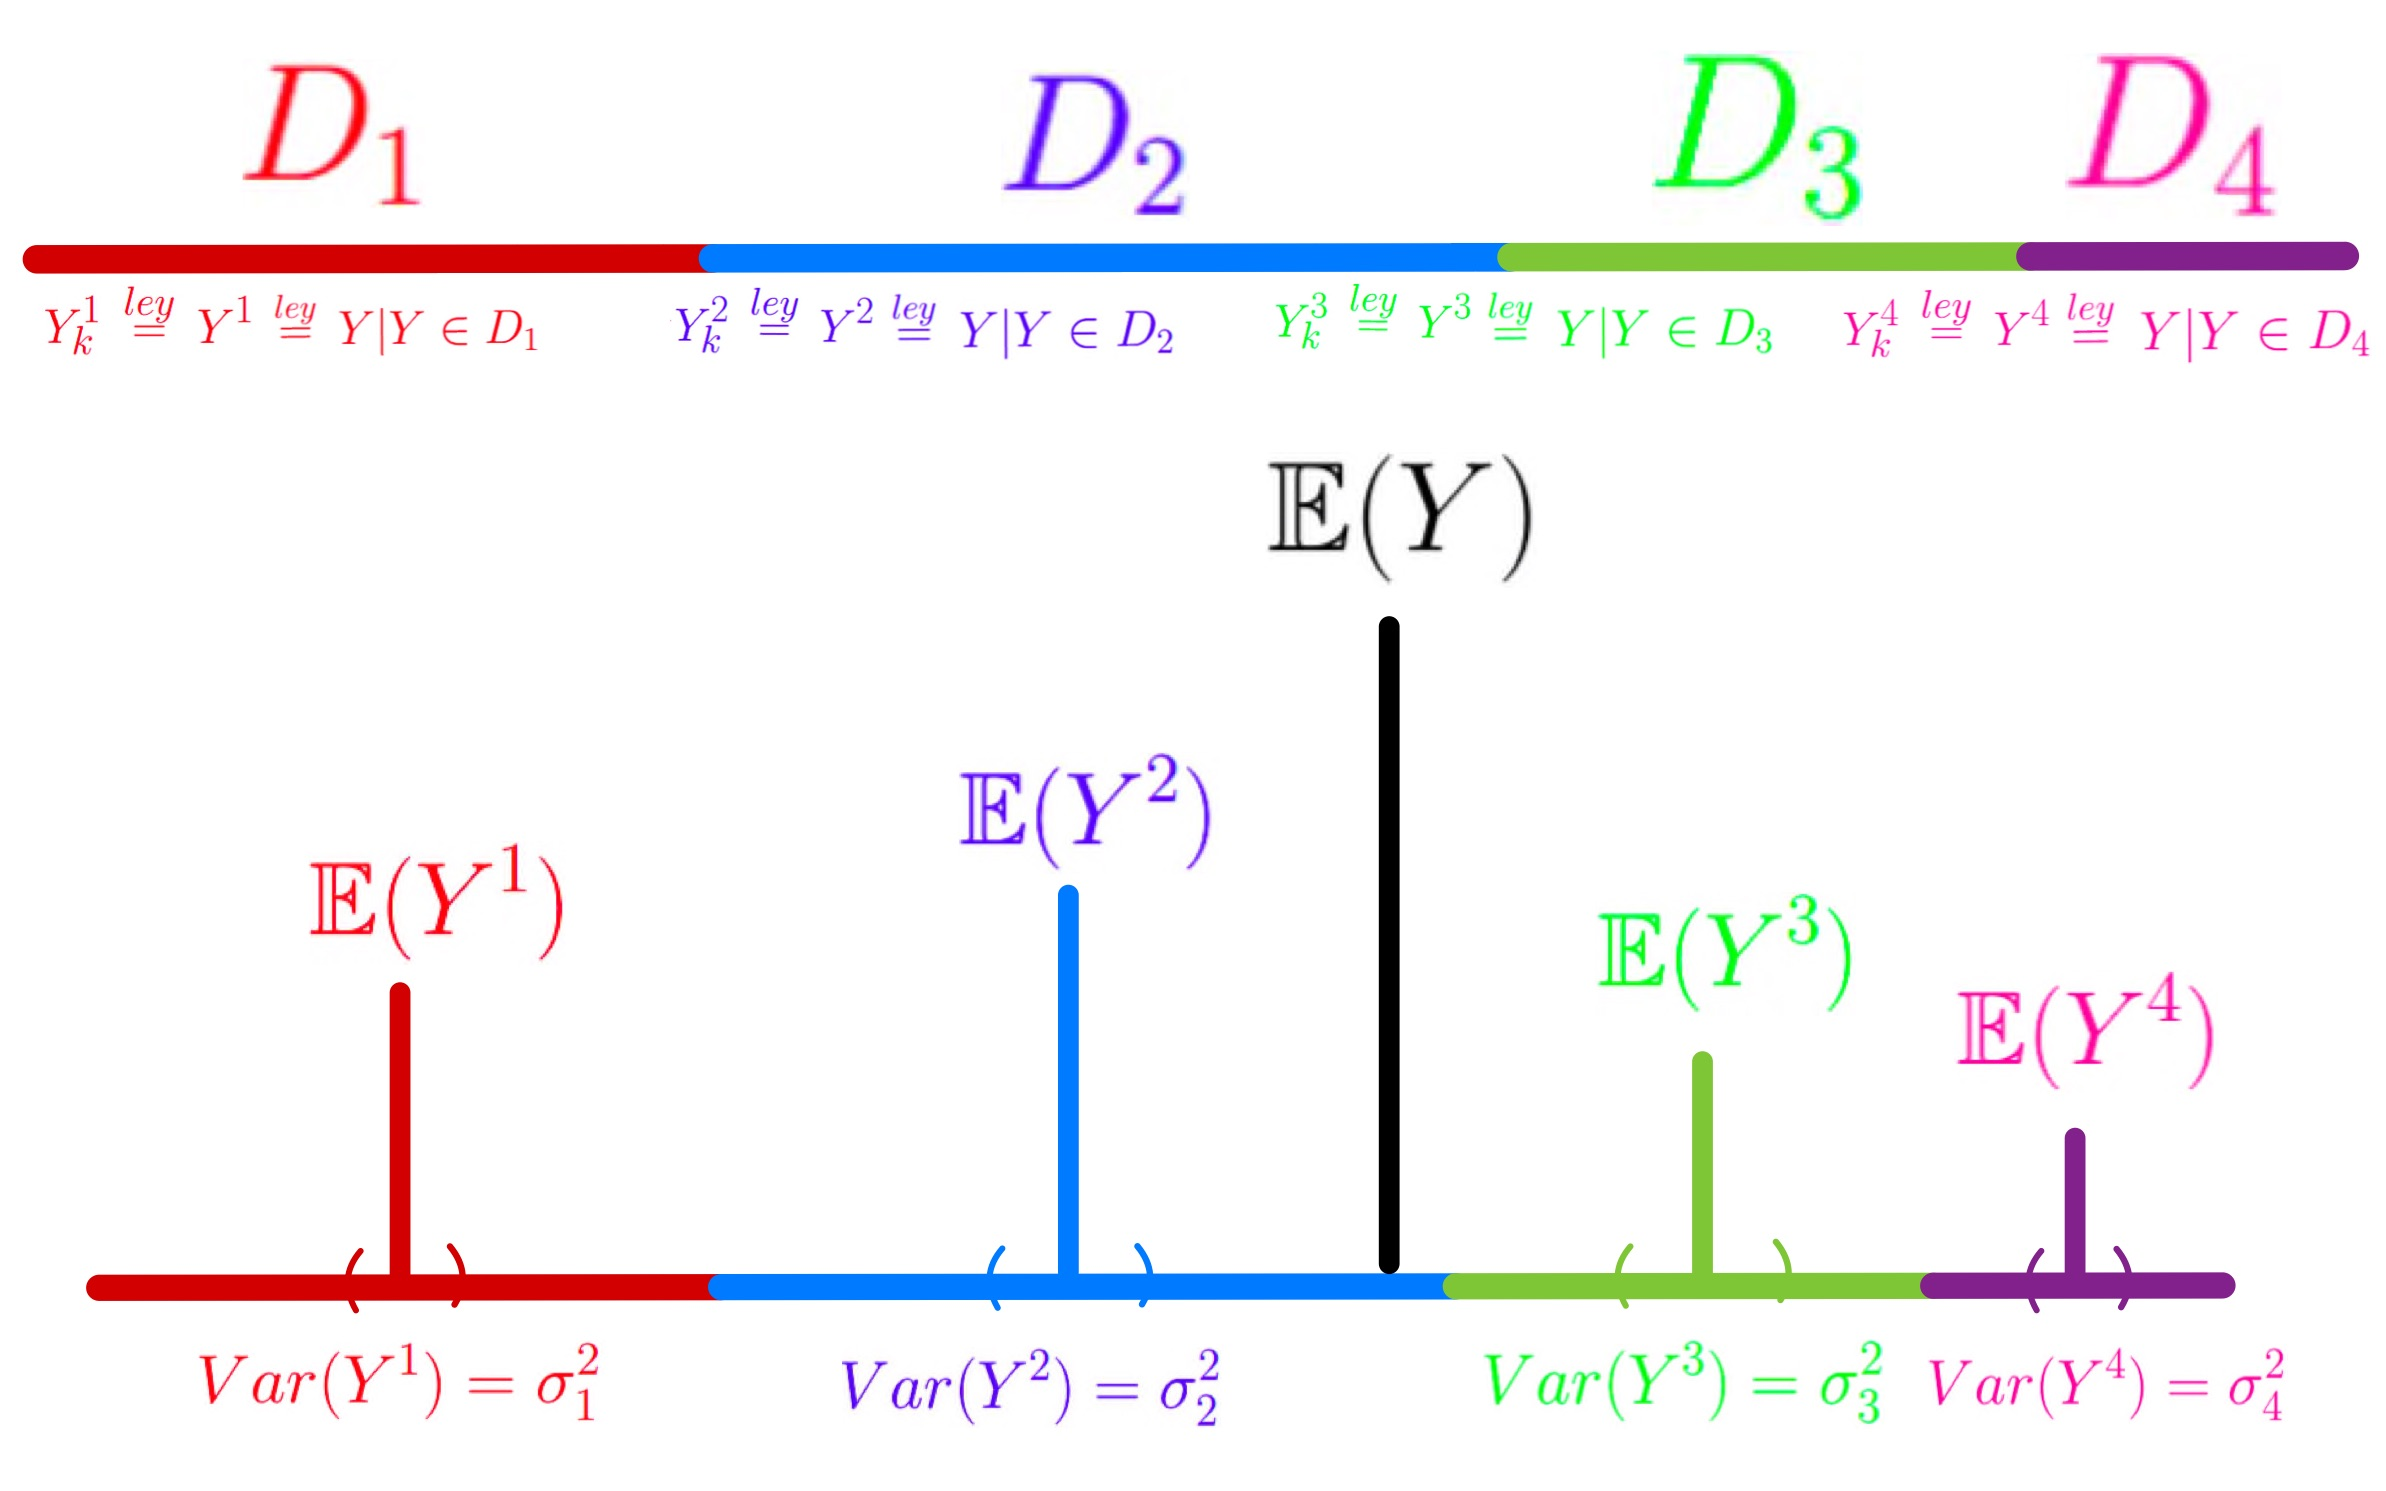
\includegraphics[scale=0.16]{img/clase_09_pag_3.jpg}
    \caption{Ejemplo gráfico de muestreo estratificado}
    \label{fig:estrat}
\end{figure}

\newp Notemos tambi\'en que  $\sum^k_{j=1}p_j\sigma^2_j= \var(\hat{Y}_n)$ si elegimos  $n_j\approx p_jn$.  Vemos entonces que, en este caso,   si $\exists j\tq\E(Y^j)\neq\E(Y)$ tendremos que $\var(\bar{Y}_n)>\var(\hat{Y}_n)$, donde $\hat{Y}$ es el estimador usual.   Dicho de otro modo, basta con que haya algún estrato para el cual la esperanza no sea igual a la esperanza de $Y$, para que se reduzca la varianza con esta elecci\'on de $n_j$'s.


% \newp Se puede escoger $n_1,\dots,n_k$ tal que $n_1+\dots+n_k=n$ de manera aún mejor resolviendo:
\newp Más aún, podemos elegir los $n_j$'s de manera aproximadamente  \'optima,  resolviendo:
\begin{alignat*}{2}
    \displaystyle\min_{n_1,\dots,n_k\geq0}& & \sum^k_{j=1}\sigma^2_j\frac{p_j^2}{n_j}\\
    \mbox{s.a.  }& \mbox{    } & n_1+\dots+n_k=n 
\end{alignat*}
suponiendo los $n_j$ reales y aplicando KKT.  Obtenemos as\'i como soluci\'on entera:
$$ n_j\approx\displaystyle n\bigg(\frac{p_j\sigma_j}{\sum^k_{l=1}p_l\sigma_l}\bigg) \, .$$
Los $\sigma_j$ a su vez, se pueden estimar con simulaciones piloto.

% $$ \color{red} \E(Y^1) \espacio \color{blue} \E(Y^2) \espacio \color{negro} \E(Y)
% \espacio \color{green} \E(Y^3)\espacio  \color{magenta} \E(Y^4)$$
% $$ \color{red} Var(Y^1)=\sigma^2_1 \espacio \color{blue} Var(Y^2)=\sigma^2_2 \espacio \color{green} Var(Y^3)=\sigma^2_3 \espacio  \color{magenta} Var(Y^4)=\sigma^2_4$$
% \big
% $$ \color{red} Y^1_1,\dots,Y^1_{n_1} \espacio \color{blue} Y^2_1,\dots,Y^2_{n_2} $$
% $$ \color{red} \overset{ley}{=}\,Y^1\,\overset{ley}{=}\,Y|Y\in D_1 \espacio \color{blue} \overset{ley}{=}\,Y^2\,\overset{ley}{=}\,Y|Y\in D_2 $$
% $$\color{green} \overset{ley}{=}\,Y^3\,\overset{ley}{=}\,Y|Y\in D_3 \espacio  \color{magenta} \overset{ley}{=}\,Y^4\,\overset{ley}{=}\,Y|Y\in D_4 $$
% $$\color{green} Y^3_1,\dots,Y^3_{n_3} \espacio  \color{magenta} Y^4_1,\dots,Y^4_{n_4} $$